\chapter{Results}
\label{sec:results}

In this chapter I will be presenting the results obtained from the validations performed in the previous section followed by the implications.

%Results and Implications
\section{Results for validation 1}
%%%%%%%%%%%%%%%%%%%%%%%%%%%%%%%%%%%%%
\begin{figure}[ht]
\centering
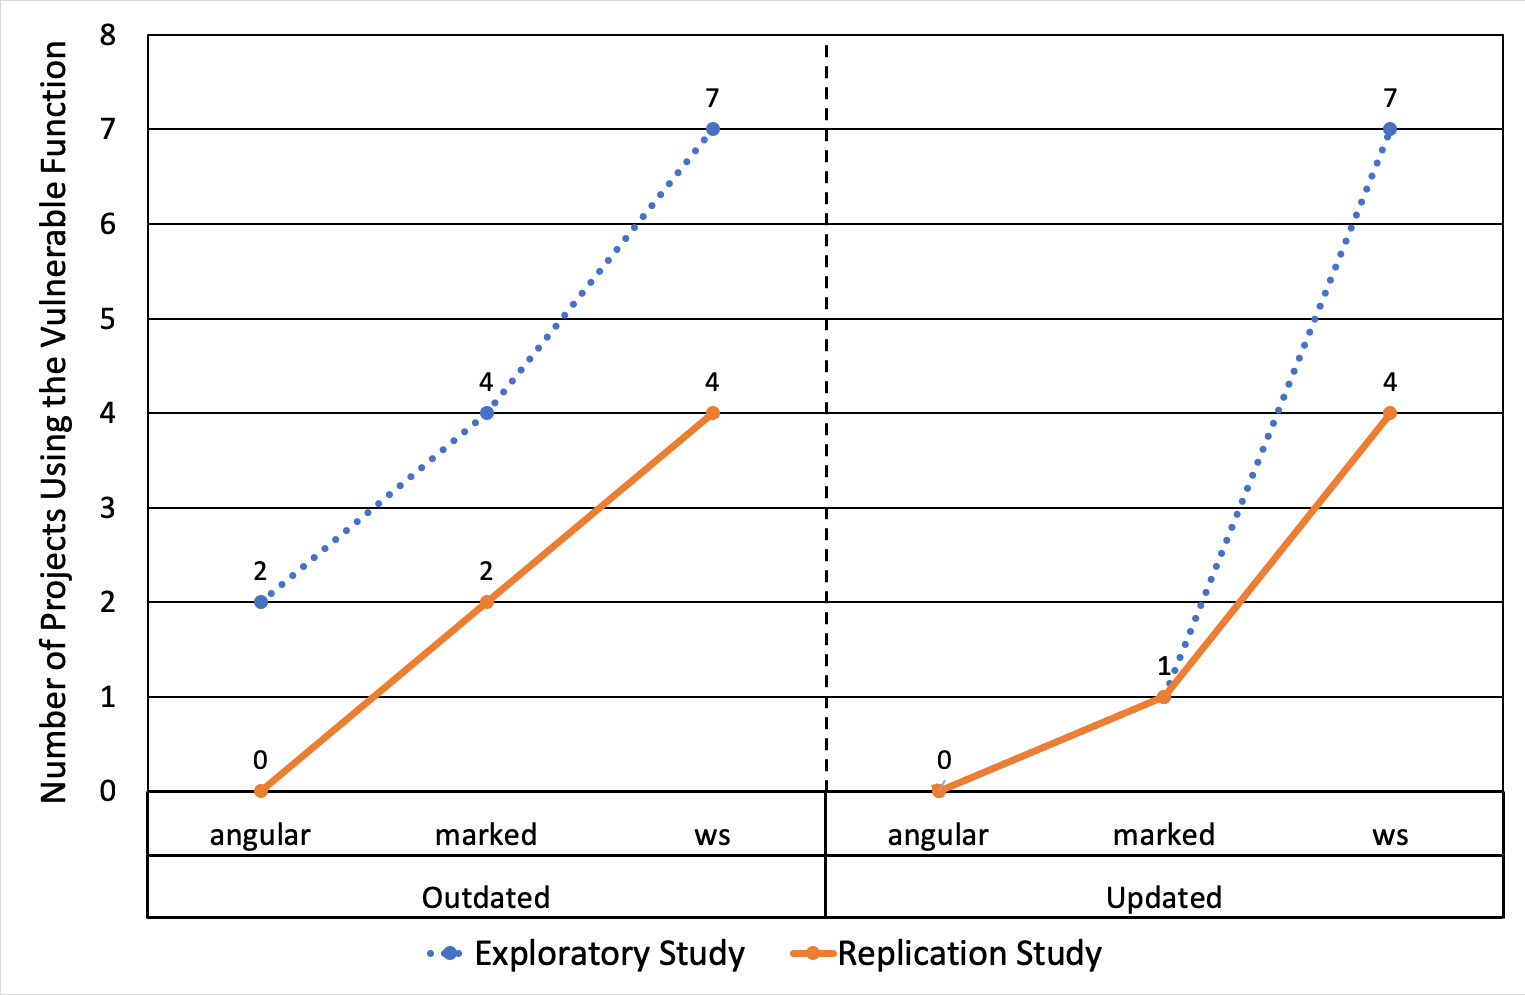
\includegraphics[width=1\textwidth]{images/studies_comp_graph3.png}
\caption{Comparison between Exploratory Study and Replication Study Results}
\label{fig:replicationResults}
\end{figure}
%%%%%%%%%%%%%%%%%%%%%%%%%%%%%%%%%%%%%
Comparing the results shown in Figure \ref{fig:replicationResults} from both studies, allowed me to calculate an estimate on the accuracy of the tool. First I obtained the base values, as those presented in the previous Chapter in Figure \ref{fig:replicationStatistics}. Once the base values were acquired I calculated the accuracy among other metrics for \tool[]. 

Table \ref{tab:replication_statistics} presents the summary of the base values and metrics calculated.

%%%%%%%%%%%%%%%%%%%%%%%%%%%%%%%%%%
\begin{table*}[ht]
\centering
\scalebox{0.8}{
\begin{tabular}{|l|c|l|}
\hline
\multicolumn{1}{|c|}{\textbf{Metric}} & 
\multicolumn{1}{c|}{\textbf{Value}} & 
\multicolumn{1}{c|}{\textbf{Description}} \\ \hline
\multicolumn{3}{|c|}{\textbf{Base Values for Calculations}} \\ \hline
n & 60 & Number of projects analyzed\\ \hline
TN & 39 & True Negatives. Predicted No and Actual No\\ \hline
FN & 10 & False Negatives. Predicted No and Actual Yes\\ \hline
FP & 0 & False Positives. Predicted Yes and Actual No\\ \hline
TP & 11 & True Positives. Predicted Yes and Actual Yes\\ \hline
\multicolumn{3}{|c|}{\textbf{Statistics Values Calculations}} \\ \hline
Accuracy & 0.833 & (TN + TP)/N\\ \hline
Miss-classification rate & 0.167 & (FP + FN)/N\\ \hline
TP rate & 0.524 & TP/(FN + TP)\\ \hline
FP rate & 0 & FP/(TN + FP)\\ \hline
TN rate & 1 & TN/(TN + FP)\\ \hline
FN rate & 0.476 & FN/(FN + TP)\\ \hline
\end{tabular}}
\caption{Base Values and Metrics from both studies results comparison}
\label{tab:replication_statistics}
\end{table*}
%%%%%%%%%%%%%%%%%%%%%%%%%%%%%%%%%%

Additionally it is important to mention that the average execution time for the function-call extraction was 0.73 seconds per project, making this approach significantly faster than the manual execution.

\section{Results for validation 2}

%%%%%%%%%%%%%%%%%%%%%%%%%%%%%%%%%%
\begin{table*}[ht]
\centering
\scalebox{1}{
\begin{tabular}{|l|l|}
\hline
\multicolumn{1}{|c|}{\textbf{Condition}} & 
\multicolumn{1}{c|}{\textbf{Number of Clients}} \\ \hline
Dependency Listed But Not Used & 98\\ \hline
Clean & 60\\ \hline
Used & 34\\ \hline
No Data Available & 8\\ \hline
\end{tabular}}
\caption{Summary of the analysis of the output generated by \tool[]}
\label{tab:impactResults}
\end{table*}
%%%%%%%%%%%%%%%%%%%%%%%%%%%%%%%%%%

Table \ref{tab:impactResults} shows the results of the analysis of the output generated by \tool[]. The results were classified in 4 main categories:
\begin{itemize}
    \item \textbf{Dependency listed but not used}. It refers to those projects where, even though the third-party library was included in the project dependencies, no method call were detected by \tool[]. I identified some of the causes for this behaviour. (i) The function-calls are outside of the scope of the tool (ii) The GitHub commit from the version analyzed contained no \textit{js} files therefore, no information could have been retrieved. (iii) The version analyzed is no longer using the third-party library but it remained in the project dependencies. 
    
    \item \textbf{Clean}. It refers to those projects where function-calls to the third-party library were detected but the function-call related to the vulnerable function was not among them.
    
    \item \textbf{Used}. It refers to those projects where function-calls to the third-party library were detected and the function-call related to the vulnerable function was among them.
    
    \item \textbf{No Data available}. It refers to those projects where no versions could be retrieved by \tool[]. Some of the causes are, (i) The library GitHub repository does not exist anymore. (ii) The developer did not include the version number in the \textit{package.json} file or did not created a tag when committing into the repository, therefore, no data could be analyzed. 
\end{itemize}

Figure \ref{fig:impactResults} shows the results of the projects where \tool[] was able to determine if the vulnerable function was used or not.

%%%%%%%%%%%%%%%%%%%%%%%%%%%%%%%%%%%%%
\begin{figure}[ht]
\centering
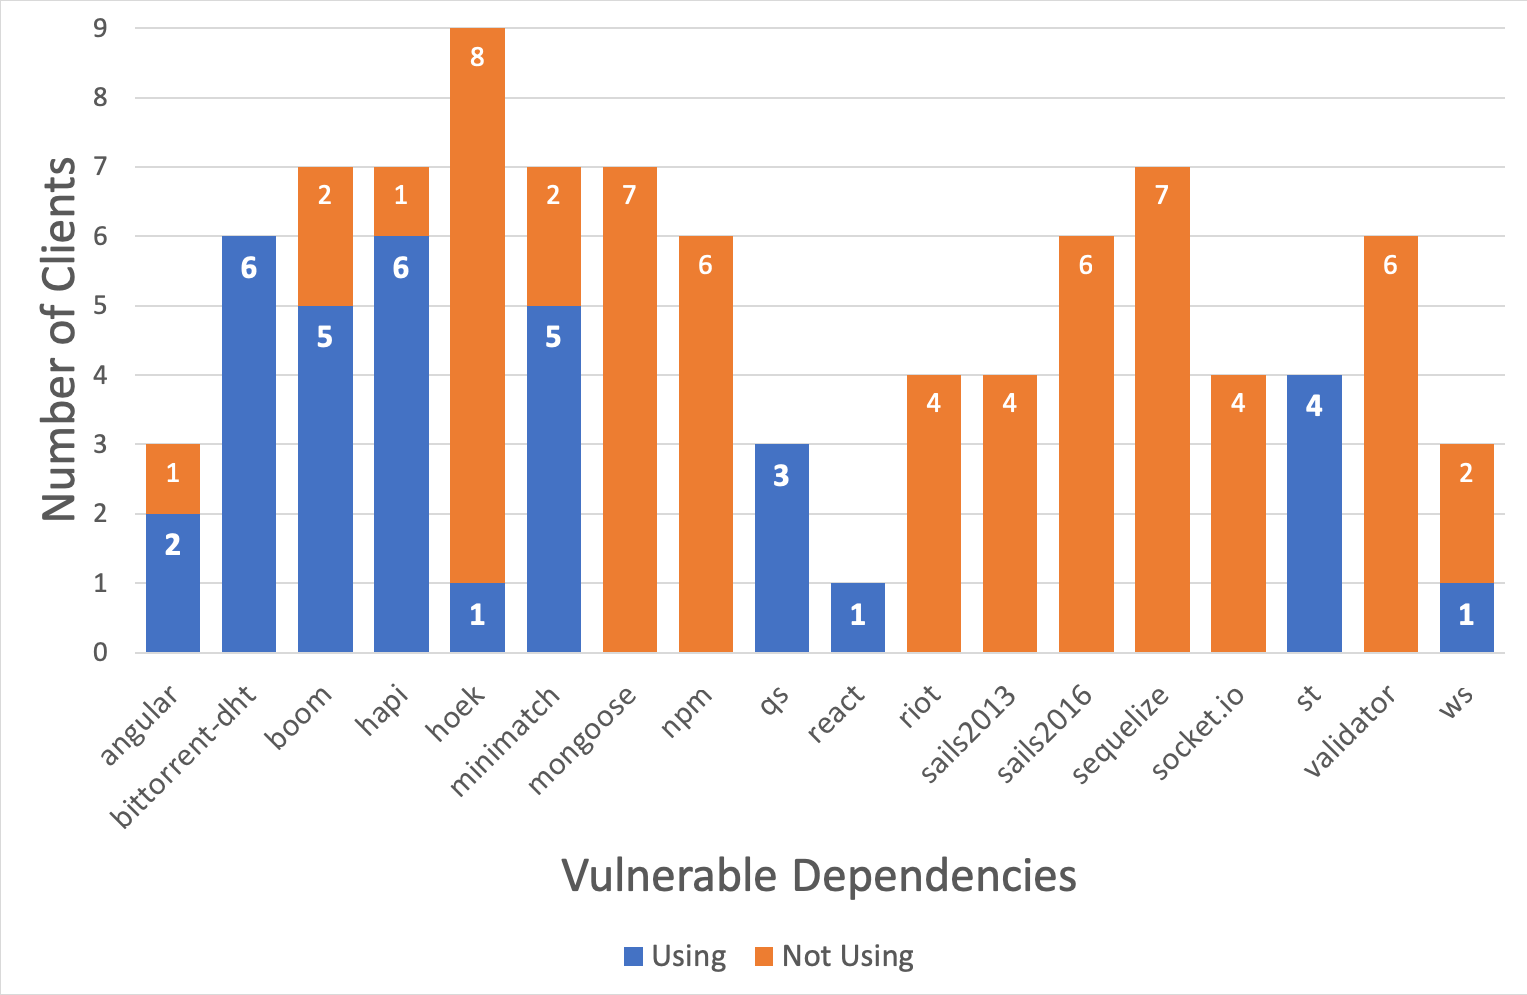
\includegraphics[width=1\textwidth]{images/impact_results.png}
\caption{Proportion of usage of vulnerable functions from third-party libraries}
\label{fig:impactResults}
\end{figure}
%%%%%%%%%%%%%%%%%%%%%%%%%%%%%%%%%%%%%

The results of this study are consistent with the previous studies where I have identified that the assumption of a project been vulnerable because it used a vulnerable library it may be an overestimation.

Detailed information of the client projects as well as the outputs generated by \tool[] to perform this study can be found on the following url: \url{https://github.com/rodrigo-e/ImpactStudy}.


\section{Implications}

After analyzing the previous results I came with the following implications:
\begin{enumerate}
    \item \textit{This case study should be expanded to other programming languages to generalize the results.}
    For this case study I am using client projects that are also npm libraries. 
    For a more rigorous study, I would like to investigate this phenomena in more generic JavaScript client projects (i.e., such as websites and frameworks written in a combination of different languages).
    
    \item \textit{Automation needs to be improved}. As shown in the results, although the tool achieved a 83\% of accuracy in comparison with the previous study, there still a gap that needs to be optimized to get better and more accurate results.
    
    For example, regarding the \textit{False Negatives}, Figure \ref{fig:falseNegativeExample} illustrates an example of a complex function-call that was retrieved manually through a regular expression search (i.e. the function \$compileProvider) in the exploratory study but was not detected by \tool[] since it is out of the current scope of the tool (i.e. those function calls that are linked to a \textit{require} statement).

%%%%%%%%%%%%%%%%%%%%%%%%%%%%%%%%%%%%%
\begin{figure}[ht]
\centering
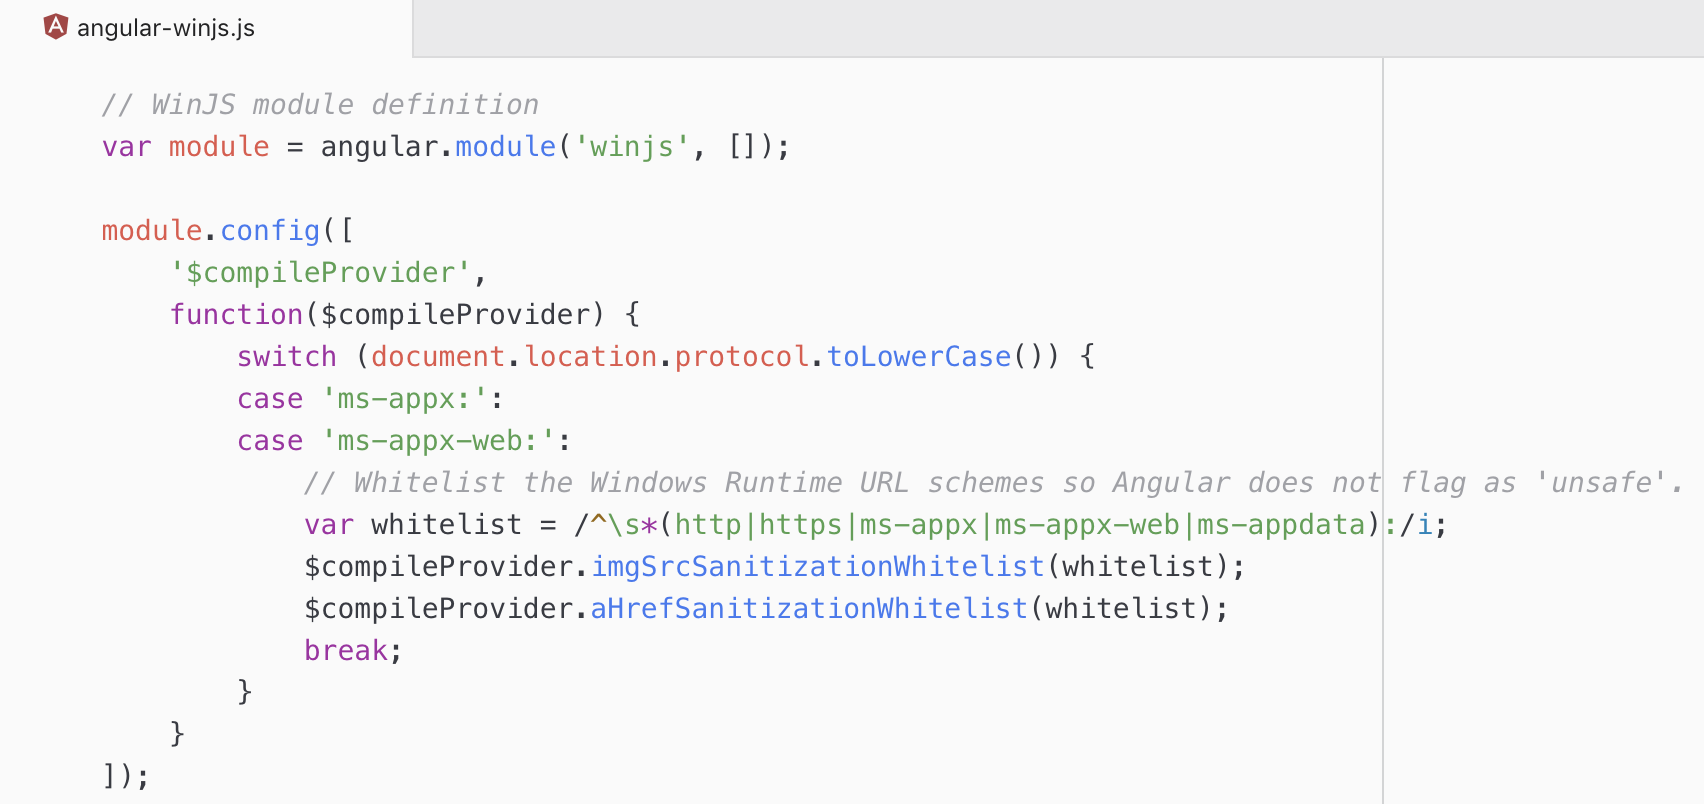
\includegraphics[width=1\textwidth]{images/false_negatives_reason.png}
\caption{Complex example of function-call not traced by \tool[]}
\label{fig:falseNegativeExample}
\end{figure}
%%%%%%%%%%%%%%%%%%%%%%%%%%%%%%%%%%%%%
    
    \item \textit{Understanding whether or not the vulnerability affects the client code will help developers better plan their library migrations.}
    I speculate that analysis to find whether or not the code is affecting the client code would be beneficial (especially for the novice developer) when making the decision to update. 

    \item \textit{Developers should be encouraged to migrate away from the vulnerable dependency, even if the vulnerable code is not being used.}
    Although there are different reasons for keeping the outdated version (i.e., fix breaks the older version or new changes are not needed), developers should be encouraged to update as soon as the fix is made available.
    Furthermore, I suggest that security only patches should be released.
    This is similar to the Debian ecosystem, where security patches are especially released and not packaged with other updates.
    I believe that this will help towards facilitating smoother library migrations.
\end{enumerate}